\documentclass{report}
\usepackage{graphicx, subfigure}
\usepackage{mathtools}
\usepackage{hyperref}
\usepackage{float}
\usepackage[section]{placeins}
\usepackage{listings}

\lstset{frame=tb,
    language=Python,
    basicstyle={\small\ttfamily},
    breaklines=true,
    breakatwhitespace=true,
    tabsize=3
}

\begin{document}

    \title{Phase Field Simulations}
    \author{Bruce Berry}
    \maketitle

    \section{Introduction}
    This report details the simulation of various molecular scale events.  The Molecular Dynamics (MD) method is used to simulate inter-particle interactions.

    \section{Background}
    Molecular Dynamics methods treat the interactions of individial atoms in a lattice to determine the behavior of a material on the atomic scale.  Atoms are arranged on a lattice representing the initial structure of the model.  The positions of the atoms are updated according to forces that result from the potentials chosen for the particle problem at hand.  By studying the changing structure of the atoms, a material's response to external forces can be understood.

    \section{Methods}
        \subsection{Copper Nanowire}
        \begin{figure}[!htb]
            \label{fig:applied-stress-partA}
            \centering
            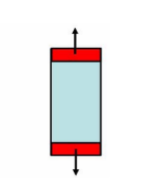
\includegraphics[width=0.4\textwidth]{applied-stress-partA.png}
            \caption{The stress Initial Condition.}
        \end{figure}
        Of interest is the simulation of a copper Nanowire's reponse to deformation.  Simulations were carried out using Nanohub's Nanowire Tensile Deformation Lab (NTDL) module.  A lattice of atoms were generated of size 20 x 20 x 130 \AA. As per the assignment's direction, the NTDL parameters were set to 8 x 8 x 36 to produce this initial condition.  The structure was set to be a free surface in each direction, with a tensile force applied to each end ~\ref{fig:applied-stress-partA}.  The tensile stress was implemented by applying a displacement of 0.02 \AA  every 20 simulation time steps. 30,000 time steps were performed.  The simulation was carried out a second time, with the cross sectional area doubled (40 x 40 x 130 \AA).

        \subsection{Collagen Stretching}
        \begin{figure}[!htb]
            \label{fig:applied-stress-partB}
            \centering
            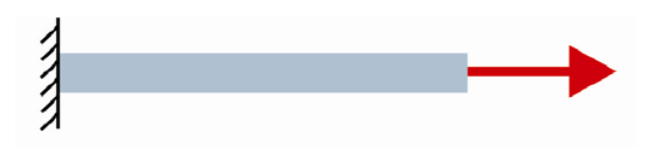
\includegraphics[width=0.4\textwidth]{applied-stress-partB.png}
            \caption{The stress Initial Condition.}
        \end{figure}
        To be investigated is the behavior of a collagen analog when subjected to a tensile force.  The software used the package stretching simulation of an alpha-helical protein domain (SSAPD).  SSAPD uses the method of Steered Molecular Dynamics (SMD) with a CHARMM force field to simulate the interaction of the molecule's componenets.  The boundary conditions are those indicated in ~\ref{fig:applied-stress-partB}.  Molecule data, including initial positions of atoms, points of fixation, and force field potentials were provided.  The SSAPD module was given the parameters according to:
        \begin{tabular}[!htb]{|l|l|l|l|}
            \hline
            DCD Freq. & Velocity & Steps & Averaging Bins \\
            \hline
            150 & 0.0005 & 150,000 & 300 \\
            \hline
        \end{tabular}

    \section{Results}
        \subsection{Copper Nanowire}



        \subsection{Collagen Stretching}


\end{document}
